\documentclass{llncs}
\pdfoutput=1
\pagestyle{plain}

\usepackage{booktabs}

\usepackage{algorithm, algpseudocode}
\usepackage{relsize}

\renewcommand{\tabcolsep}{2pt}

\setcounter{secnumdepth}{3}


\renewcommand{\algorithmiccomment}[1]{/*#1*/}
\usepackage{epsfig, endnotes, url}
\usepackage{color, cite, graphicx}
\usepackage{mathtools, amsmath, amsfonts}
\usepackage{diagbox, booktabs, colortbl}
\usepackage{multirow, subcaption}
\usepackage{breakurl, listings, framed}
\usepackage[hidelinks]{hyperref}
\usepackage{xspace, slashbox, enumitem, array}
\DeclareMathAlphabet{\mathcal}{OMS}{cmsy}{m}{n}

\captionsetup[subfigure]{justification=raggedright}

\newcolumntype{?}{!{\vrule width 1pt}}

\captionsetup{compatibility=false}
\def\UrlBreaks{\do\/\do-}
{\renewcommand{\arraystretch}{1.2}
\makeatletter
\newcommand{\@chapapp}{\relax}%
\makeatother

\usepackage[title]{appendix}

\newcommand{\tabitem}{~~\llap{\textbullet}~~}

\newcommand{\ignore}[1]{}
\newcommand\ghada[1]{\nbc{GA}{#1}{teal}}
\newcommand\david[1]{\textbf{\textcolor{blue}{[david] #1}}}
\newcommand\derek[1]{\textbf{\textcolor{green}{[derek] #1}}}
\newcommand{\fake}[1]{{\color{magenta} [fake: #1]}}
\usepackage{array}
\newcolumntype{P}[1]{>{\centering\arraybackslash}p{#1}}

\newcommand\stakeescrow{\textsf{StakeEscrow}\xspace}


\begin{document}

\title{\Large \bf Confirm Activity in the NuCypher Network \\
(WIP)}
\author{Ghada Almashaqbeh}

\institute{NuCypher \\
\email{ghada@nucypher.com}}
\date{} % delete this line to display the current date



\maketitle

\begin{abstract}
In this document we study the confirm activity problem in the NuCypher network. This problem is concerned with devising secure techniques that allow Ursula to prove being online and responsive during any time period. We consider two flavors of the problem based on the network operation stage, namely, confirm availability and confirm service activity. The former is about confirming that Ursula is available all the time and replies to all Bob requests, while the latter is about proving that an Ursula has served a specific number of distinct re-encryption requests within a given period. We present several potential solutions for each of these types, discuss the characteristics of these solutions with respect to their security guarantees and efficiency, and provide recommendations to when each of them should be used.
\end{abstract}

\section{Introduction}
\label{intro}
The NuCypher network~\cite{nucypher,egorov2017nucypher} is a decentralized key management system, encryption, and access control service. It uses threshold proxy re-encryption, namely, the Umbral scheme~\cite{umbral2018}, to delegate access to encrypted data through a public network. This network is composed of semi-trusted re-encryption service-providers, or Ursulas, that implement access control policies created by data 
owners, or Alices. Alice supplies each Ursula with re-encryption keys allowing a quorum of Ursulas to transform 
ciphertexts encrypted under Alice's public key into ciphertexts encrypted under the delegatee's, or Bob's, public key. This enables the latter to decrypt the ciphertext without revealing anything about the decryption keys or the raw data to the intermediate service-providers. 


Joining the NuCypher network is governed by consensus rules defining the service setup and the monetary incentives paid to provide the service. In order to join the system, Ursula needs to stake an amount of NU tokens (the native token of the network) for a specific period which will be released when the pre-specified staking period is over. Alice chooses an Ursula to hold an access control policy with a probability proportional to the stake this Ursula pledged in the system. Therefore, the stake value influences the service load an Ursula may receive. This stake is also used to punish Ursula financially, by forfeiting part of it for detectable malfeasance. 


Alice uses the network by creating an access control policy to be implemented by a set of Ursulas. This policy specifies the re-encryption key fragments each Ursula will need to answer requests coming from Bob(s), as well as the duration of the policy, which is basically the timeframe during which Bob is authorized to access Alice's data. Furthermore, the policy contract requires Alice to lock an amount of Ether that will be used by the network to pay Ursulas for providing the re-encryption service. As noted, Alice is not exposed to the NU token. All that she needs is an Ethereum wallet, awareness of the NuCypher network architecture to select Ursulas, and knowledge of the NuCypher rules with respect to preparing access control policies.


Bob, on the other hand, does not deal with currency in the system at all. He interacts with the storage network to retrieve the encrypted data, and with Ursulas in the NuCypher network to request the re-encryption service after which he will be able to access the raw data of interest.


\paragraph{\bf Rewards and activity monitoring in the NuCypher network.}
Ursulas are rewarded for their re-encryption service by using two sources; the first is the service fees collected from the policy owner Alice, while the second is a subsidy in the form of newly minted NU tokens distributed on a schedule enforced by the NuCypher protocol. The latter will be provided during the early stage of the network operation to encourage Ursula's participation and sustain their operations in lieu of a mature fee market.


Currently, the subsidy size in each round or period is computed for each Ursula based on the size of her stake and duration of commitment to the network, and provided that she confirms to be online during this round. Confirming the status of being online is done by calling a simple function in one of the NuCypher contracts, which is like a signal that the calling Ursula is online. Similarly, for service fees, Ursula collects part of the Ether locked by Alice during the policy's duration in proportion to the number of periods up to that point in which Ursula has confirmed her online status.


\paragraph{\bf Motivation.} Although rewards computation and activity monitoring are reasonable for the first iteration of the network, we acknowledge that it suffers from two main problems:
\begin{itemize}
\setlength{\itemsep}{0pt}
\item Confirming being online is flawed in the sense that the function call that Ursula makes does not require any input or proofs on providing the service, or even being online and responsive. Ursula can stay offline the majority of the time and not respond to Bobs' requests, then come online merely to call this function. This allows Ursula to collect both subsidy and fees without doing all (or even most) of the necessary work. Even worse, Ursula will be able to get her stake back once it unlocks.

\item The revenue computation (both fees and subsidy) is agnostic to the number of requests Ursula serves. Thus, an active Ursula who may serve a huge number of re-encryption requests, and one who does not receive any requests (or more importantly, a malicious/lazy Ursula that does not answer Bob's requests), will both collect the same amount of revenue if they hold identical policies.
\end{itemize}


Nonetheless, Ursula has an economic incentive to log her availability and provide a satisfactory level of service. If she ``cheats" she will risk devaluing her stake since the network will be less useful to users who will leave and cease paying fees. However, we recognize the long-term need for a more intelligent and specialized technique to hold Ursula accountable and prevent her from cheating the system. Then we need to adapt the subsidy and fee computation accordingly to factor in the amount of delivered service, and potentially punish Ursulas if it is insufficient.


\paragraph{\bf Problem statement.}
The confirm activity problem is defined differently based on the network operation stage. In the first 5 to 8 years after launch, when subsidy rewards are still distributed, we are concerned with the availability of Ursulas and their willingness to serve all requests coming from Bob. In other words, regardless of the number of requests served, the revenue total value (both subsidy and fees) will be computed based on the length of time during which Ursula is online and well-behaved. 


On the other hand, in later stages, when subsidies disappear and the only revenue comes from fees, confirm activity will be tied to providing the re-encryption service, in the sense that the payment will be partially computed based on the amount of service provided. This requires Ursula to confirm its activity by proving that she served a given number of distinct re-encryption requests during a given period. 


To make the distinction clear, we refer to the first as \emph{confirm availability}, and for the second as \emph{confirm service activity}.


\paragraph{\bf Contributions.}
In this document, we introduce several solutions for both forms of confirming activity. These solutions differ in the trust, security guarantees, interactivity, and efficiency. 


For confirming availability, we employ a detect-and-punish approach embedded within an optimistic service monitoring process. This means that it is only invoked when Bob complains that an Ursula is unresponsive. The proposed solution labels Ursulas as working and gateway Ursulas. The former are contacted in a regular way to handle the re-encryption service, while the latter act as challengers that are contacted only when there is a complaint from Bob so they will attest whether a working Ursula is indeed unavailable. If that is the case, a quorum of gateways (who have challenged the working Ursula and found her unresponsive) will collectively sign a proof-of-unavailability that will cost the misbehaving working Ursula part of her stake. We discuss several aspects related to gateway selection and a variety of potential attacks on this approach along with mitigation techniques.


For confirming service activity, we devise three solutions that allow producing a proof attesting to the statement \emph{``An Ursula has served $\omega$ distinct requests correctly"} for some positive integer $\omega$ representing the number of served requests. These solutions are refereed to as zero knowledge proof-based (ZKP-based), committee-attestation, and commit/challenge/open-based. 


For the \emph{ZKP-based} approach, we utilize the fact that in our network each Ursula already produces a ZKP attesting to the correctness of each re-encryption request she performs~\cite{umbral2018}. Our solution is to aggregate the proofs of all served requests within a round into one proof attesting to the above statement. This accumulation can be done by using generic techniques like proof carrying data (PCD)~\cite{chiesa2010proof} or incrementally verifiable computation (IVC)~\cite{valiant08}. An alternative, possibly more efficient approach, is to view the above statement as an instance of arithmetic circuit satisfiability problem and combine it a highly efficient ZKP system, e.g.,~\cite{bunz18}. That is, build a circuit that takes the set of correctness proofs and their count $\omega$ as inputs. If the number of correct distinct proofs equals to $\omega$, i.e., the circuit output 1,  then a valid proof will be produced. Ursula can submit this proof to the network to claim her payments. 


As for the \emph{committee-attestation} approach, it shares a similar theme to confirm availability solution mentioned previously. For each round, a committee of Ursulas (and possibly outsider verifiers) is elected to attest for the work load an Ursula served. In detail, the working Ursula sends all Bob requests she served along with the correctness proofs to this committee. After verifying all the proofs, the committee collectively signs the \emph{``An Ursula has served $\omega$ distinct requests correctly"} statement, while replacing $\omega$ with the actual number of served requests. The committee (or the working Ursula) submits the signed statement to the network so the working Ursula can claim her payments.


For the \emph{commit/challenge/open} approach, we introduce a mechanism inspired from the Merkle tree-based ZKP system proposed in~\cite{dottling19}. For each round a working Ursula constructs a Merkle hash tree of all served requests and their correctness proofs. Then, she uses the root as a random beacon to be fed into an iterative hash process to select $n$ leaf nodes at random to open them (i.e., these are the challenges). Ursula signs the Merkle tree root and the activity proof will be composed of the signed root, the challenge leaf nodes along with their openings, and membership paths of the challenge leaves. Ursula sends this proof to either a sidechain (maintained by round-selected committee) or to the main network to verify. Once verified, Ursula will be rewarded with the service payment.


Lastly, we discuss the trade-offs of each of these solutions in terms of security guarantees, assumptions, and efficiency. We also outline some recommendations regarding which solution should be used at what stage of the network operation. 


\paragraph{\bf Organization.}
We begin with outlining the adopted threat and network model, in Section~\ref{threat-network-model}, followed by an overview of some of the cryptographic primitives that we use in Section~\ref{prelim}. Then, we present the proposed solutions for confirm availability in Section~\ref{confirm-availability} and those for confirming service activity in Section~\ref{confirm-service-activity}. Lastly, we briefly discuss the trade-offs and requirements of each of these solutions along with some usage recommendations and future work directions in Section~\ref{discussion}.
\section{Confirm Availability}
\label{confirm-availability}
In this section, we present a solution for confirming availability of 
Ursulas. As mentioned before, in the early operation stage of the network we only 
require Ursulas to be online and responsive to the re-encryption 
requests issued by Bob. 


We introduce the design details of our solution, after which we discuss some potential security attacks and how to address them.


\subsection{Optimistic Challenge-based Approach}
The proposed solution is centered around two important concepts: requiring minimal 
changes to the current network implementation, and minimizing the additional overhead. \\


\noindent{\bf Discovering Working Ursulas.} Recall that in the NuCypher network, Bob receives a map from Alice containing 
the set of Ursulas that has the key fragments needed to implement the access control policy. 
When issuing a re-encryption request, Bob uses this map (in association with the network discovery protocol) to reach each of these Ursulas and obtain 
the service. 


In particular, in the NuCypher network there is a separation between the role of a staker and a working Ursula. All stakers' Ethereum addresses, along with their stake values, are recorded in one of the NuCypher network smart contracts, namely, the \stakeescrow contract. Each of these stakers will be tied, or bonded, to a working Ursula to provide the re-encryption service by having its address listed next to the staker's address. 


The \stakeescrow contract does not contain any information about how to reach a specific working Ursula. Thus, the map that Bob receives includes only the Ethereum addresses of the working Ursulas. To allow the parties to communicate with each other, each participant, i.e., Alice, Bob, Ursula, employs a discovery protocol (more like a gossiping protocol) to discover the IP addresses and ports of the working Ursulas in the network.  


The discovery process also includes retrieving the keypair a working Ursula uses for the re-encryption service purposes. We call this keypair a stamp, and we require an Ursula to use her stamp when signing all messages related to the proposed confirm availability protocol. \\


\noindent{\bf Optimistic Ursula Challenging.} Once Bob discovers the working Ursulas listed in the policy map, he can connect with each of them and start issuing service requests. As noted, this communication is one-to-one meaning that no other Ursulas (or any 
NuCypher network participant) mediates the communication between Bob and working  
Ursula. This in turn means that no one can attest to whether Ursula has responded if Bob 
complains later that he was not served.


The main idea is to add a mediator, or potentially a witness, in the service process (if needed) to monitor a specific working Ursula and challenge its responsiveness. Hence, it is an optimistic protocol invoked only when Bob complains about not receiving the service. In detail, for each round (where a 
round is the time needed to mine a block or several blocks on the blockchain) a set of Ursulas is selected at random. We call these gateway Ursulas. Bob contacts a working Ursula asking for the re-encryption service as usual. 
If this Ursula does not respond, Bob complains to a gateway about it. At this point, the gateway will act as an intermediary and forwards Bob's request to this working Ursula on behalf of Bob and waits for the answer. If no answer is received, this gateway will trigger other gateways to perform the same process, i.e., forward the request on behalf of Bob and wait for an answer. If the working 
Ursula is still unresponsive, these gateways will collectively sign a proof-of-unavailability, which is basically a statement saying that the working Ursula was contacted by these gateways and she did not respond, and publish it through the \stakeescrow contract (see Section~\ref{cosi} for an overview of collective signing). Once the proof-of-unavailability is verified, part of the working Ursula's stake will be slashed as a punishment. \\


\noindent{\bf Gateways Selection.} For each round a set of $n$ gateways Ursulas will be selected. A proof-of-unavailability will be accepted by the network if it is signed by at least $t$ gateways among this set (this threshold is a relaxation of requiring all gateways to sign since it could be the case that not all of them are active). 


A simple idea to select the gateways is to use a high entropy source of randomness to obtain a random beacon for each round. Then feed this beacon into an iterative hashing process. After each iteration, map the hash to a working Ursula index as listed in the \stakeescrow contract. That is, the working Ursula bonded with the first staker listed in the contract has index 0, the next has index 1, etc. Then, rehash the previous hash and map the output to an index, and so no. In case of a collision, i.e., an already selected index is produced again, discard it and proceed to the next hash iteration. This process is repeated until a set of distinct $n$ indices is computed. 


Note that the selection process may contain Ursulas for which Bob does not have a contact information. Hence, Bob has to discover these Ursulas before being able to submit a complaint. To reduce the delays, and as outlined earlier, Bob starts with complaining to one gateway and involves the rest if the working Ursula does not respond to the challenge from this gateway. Hence, Bob can start with a gateway that he already knows how to reach (if any) and in the meantime works on discovering the rest of the selected gateways (if he does not already have their contact information).


Furthermore, the above protocol assumes working in the random oracle model, meaning that hash functions are modeled as random oracles. Thus, the iterative hashing process selects at random the working Ursulas. Although, we believe this is sufficient for our purposes, this can be replaced with more sophisticated approaches to produce random strings (that are then mapped to indices), e.g., a verifiable random function~\cite{micali1999verifiable}. We leave this as part of our future work in case we decide to pursue this path. 


As for the high entropy source of randomness, there are several potential approaches here. We can rely on an external source, e.g., the NIST random beacon~\cite{nist-beacon} or even a combination of multiple sources, for that. Or we can work also in the random oracle model and assume that block hashes are drawn from a uniform distribution, and thus, use the block hash as a random beacon. In particular, for the current round, the hash of the block that was mined $y$ rounds ago is used ($y$ is the confirmation interval in the underlying cryptocurrency system). Alternatively, and to avoid the random oracle assumption, we can use randomness extractors to produce a high entropy beacon from the block hashes which itself could be low entropy~\cite{bonneau2015bitcoin}. \\


\noindent{\bf Proof-of-unavailability processing.} As mentioned previously, a proof-of-unavailability against a working Ursula is a statement stating that this Ursula was unavailable during a specific round signed by at least $t$ gateways out of the $n$ gateways selected for that round. Such a proof is submitted to the \stakeescrow contract and is verified as follows:
\begin{itemize}
\item Produce the list of gateways selected for the current round. This is done by using the same process described previously.

\item Verify the collective signature over the signed statement (see Section~\ref{cosi}).

\item If everything is fine, the \stakeescrow contract revokes part of the stake bonded to the working Ursula as a punishment.
\end{itemize}


Note that the above assumes that the \stakeescrow contract is aware of the gateways' stamps (or keys) that are used in signing the proof-of-unavailability. This can be done by either expanding the staker list in the contract to contain not only the Ethereum addresses of working Ursulas, but also their stamps. Another option is to piggyback the stamps (signed by using the key corresponding to the working Ursula's Ethereum address) with the proof-of-unavailability. A more simpler, and efficient, option is to sign the proof-of-unavailability by using the key corresponding to the working Ursula's Ethereum address in the first place, and thus, the \stakeescrow contract will not need an additional information. Which option to use depends merely on efficiency considerations. \\


\noindent{\bf Quantifying the Financial Punishment or Slashing Value.}
A question that comes to mind is how much should be revoked from Ursula's stake once a proof-of-unavailability is approved? Quantifying this amount should be driven by two factors; the unavailability duration and the utility gain (or profits) of this cheating behavior in terms of the collected fees and inflation rewards for that duration.


Accordingly, we can compute this value to be equal to the fees and inflation rewards that an Ursula is supposed to receive in a round (recall that a round is the time needed to mine a block or several blocks on the blockchain). Hence, the working Ursula will, first, lose her fees and inflation rewards from the network, and second, lose the same amount from her stake. Such a loss will take place even if a single proof-of-unavailability is received against a working Ursula within a round. In fact, the \stakeescrow contract will process only one proof against a working Ursula per round to reduce computational costs in the system. \\


\noindent{\bf Working Only During the Challenge Phase.}
A potential issue under the proposed optimistic scheme is that a working Ursula may operate only during the challenge phase. That is, she ignores any fresh request coming from Bob, and just replies afterwards when receiving the same request again (i.e., when it is forwarded by the gateways during the challenge phase). 


We argue that such a behavior is not a practical issue since a rational Ursula will be online eitherway to monitor whether this is a challenge phase or not, and that the amount of work needed to respond to a re-encryption request is minimal. Hence, there is no incentive at all to follow this strategy, meaning that a rational Ursula will act honestly. \\


\noindent{\bf DoS Attacks.} 
Another potential issue is exploiting the unavailability complaints to perform a DoS attack against the gateways and working Ursulas. In detail, Bob may lie and issue complaints against working Ursulas even though they are responsive just to slash their stakes. Or an attacker may replay these complaints, or issue them on behalf of Bob, to slash a working Ursula. Or the goal could be to overwhelm the gateways with the challenge process and make them unavailable to perform the re-encryption service (recall that the gateways are originally working Ursulas in the NuCypher network).


This issues can be handled using a collection of techniques as follows:
\begin{itemize}
\item Require Bob to sign all the complaints (so no one can impersonate Bob unless they know his signing key), and include a timestamp or a sequence number in each of them (to ensure freshness and prevent replay attacks).

\item Increase the cost of issuing complaints. That is, require Bob to do some work in order to produce a valid complaint (in a similar way to proof-of-work, i.e., produce a hash over the complaint with specific number of leading zeros).
\end{itemize}


\noindent{\bf Unresponsive Gateways.}
A third issue that we may encounter in the proposed solution is that the gateways themselves could be unresponsive. This will stall the challenge phase and make it infeasible to prove that some working Ursula is unavailable. We believe that such an issue will be organically handled by the network. That is, the larger the number of Ursulas in the network, the higher the chances of having more honest Ursulas. By increasing the number of selected gateways $n$, and given that the selection process is random, the chances of having at least $t$ honest gateways in a round will be high.


Another mechanism is to incentivize the gateways to do the work in the form of a small fee paid out of the revoked stake.


It could be the case that all gateways in a round are responsive (although we believe that the probability this happens is very low). In this case, it could be viable to perform the challenge phase in a recursive way. In other words, Bob can send an unavailability complaint against the gateways of the current round to the gateways of the previous round. The previous round gateways will in turn challenge the current round gateways by forwarding Bob's complaint to them and sign a proof-of-unavailability if no response is received. 


\section{Confirm Service Activity}
\label{confirm-service-activity}
In this section, we present potential solutions for the confirm service activity 
problem. The goal is to come up with provably secure solutions that allows an 
Ursula to prove that it has served a given number of distinct re-encryption 
requests within a given period. 


The rest of this section discusses the proposed solutions along with an analysis of 
their security and efficiency aspects. Lastly, the section concludes with directions of 
future work on the confirm service activity issue.


\subsection{Potential Solutions}
\label{solutions}
This section outlines several potential solutions for how to let Ursula prove 
that she served a given number of distinct requests in a publicly verifiable way. 
One of these solutions, the PCD-based one, is still a work in progress. The goal 
is to share the high-level idea of each of these solutions and to chose the best one,
after we define the meaning of best, to be adopted by the NuCypher network.


\subsubsection{PCD-based Scheme.}
The main idea here is to adapt the PCD framework so that Ursula
can combine the correctness proofs she computes for Bobs' requests in a single proof 
attesting to the following fact: ``Ursula has served $\omega$ distinct re-encryption 
requests correctly." 


Thus, in this setup, there is only one computation party, or prover, namely, Ursula. 
For each round, where a round could be the time needed to mine a block on the 
blockchain, Ursula starts with input $x_1$, which is a signed and fresh request
from Bob. It answers this request with $cFrag_{x_1}$ and produces a correctness 
proof $\pi_1$ as defined in the Umbral scheme, in addition to another correctness 
proof $\hat{\pi}_1$ that will be used in the PCD composition. Then, when the next request $x_2$ arrives, 
which is the input for the next step in the computation, Ursula answers 
this request as before and produces $cFrag_{x_2}$ and a correctness proof $\pi_2$, then 
it uses $(x_2, cFrag_{x_2}, \pi_2)$ and the previous proof $\hat{\pi}_1$ to produce $\hat{\pi}_2$. 
$\hat{\pi}_2$ does not only 
attest to the correctness of $cFrag_{x_2}$, but also attests to the fact that Ursula has served 
two valid distinct requests until now. The same process is repeated until the end of the 
round to produce a single proof $\hat{\pi}_{\omega}$ along with the number of 
served requests $\omega$. Figure~\ref{pcd-based-sol} depicts 
this process pictorially.


\begin{figure}[h!]
\centerline{
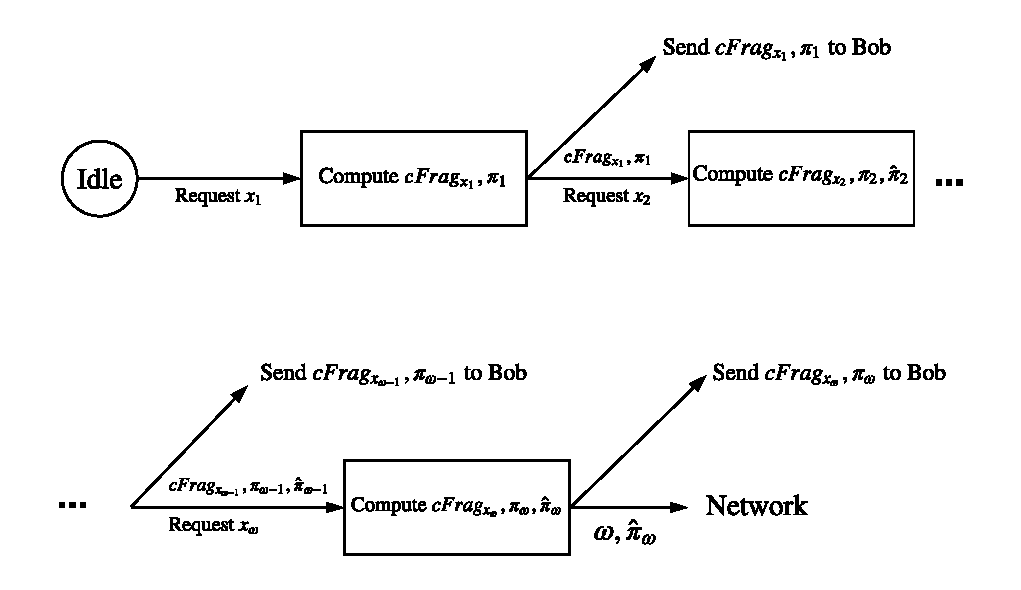
\includegraphics[height= 0.7in, width = 1.0\columnwidth]{figures/pcd-based-sol.pdf}}
\caption{PCD-based solution diagram. Ursula starts a round in the idle state. When 
the first request arrives, Ursula responds to the request and starts composing the 
proofs as new requests arrive. At the end of the round, Ursula announces the number of 
served requests and a single proof attesting to its claim to the network. }
\label{pcd-based-sol}
\end{figure}


The final proof will be processed by the contract that governs Alice's policy. A valid proof 
allows Ursula to claim fees out of Alice's Ether escrow as a payment for $\omega$ re-encryption  
requests. 


The above is a high level description of the idea. However, more time is need to 
understand PCD and SNARKs in order to come up with a concrete construction 
(if possible). Please see Section~\ref{future-work} for more information.


\subsubsection{CoSi-based Scheme.}
This solution utilizes the idea of collective signing by electing a committee 
that will sign a report submitted by a specific Ursula after verifying that 
the report supports the claim that ``Ursula has served $\omega$ distinct 
re-encryption requests correctly." 


At a high level, the scheme works as follows. For each round, a working Ursula keeps 
a full record of all the requests that she served during the round. These 
include the signed requests received from Bob(s), and the produced $cFrag$ 
and the correctness proof $\pi$ (as in the Umbral scheme) for 
each request. At the end of the round, a committee of $t$ Ursulas is 
elected, where $t$ is a small integer, e.g., $t = 5$. The working Ursula 
initiates the CoSi protocol to sign the message $m$ stated above while 
replacing $\omega$ with the actual number of served 
requests in the round. This Ursula sends $m$ along with the full report to 
each member in the committee. Each member Ursula (i.e., member in the 
elected committee) verifies $m$ by checking the report as follows:
\begin{enumerate}
\setlength{\itemsep}{0pt}
\item Check that each request is distinct by checking the sequence 
number of the request (or any value that is used for freshaness), and valid by verifying Bob's 
signature over the request. (Here the policy will contain Bob's public 
key to allow the committee use the right verification key.)


\item Verify the correctness of each $cFrag$ as in the Umbral 
scheme.

\item Check that the value of $\omega$ inside $m$ agrees with the 
record.
\end{enumerate}


If everything is fine, each member of the committee and the working 
Ursula finalize the CoSi signing protocol as described in Section~\ref{cosi}. 
At the end, the working Ursula publishes the collective signature, which can be 
verified using the accumulated public keys of the cosigning Ursulas.


\paragraph{On the committee election.} This can be done
by using some deterministic computation over a block hash and mapping
the output to Ursulas' public keys. So the selection is not determined by the
working Ursula to prevent any potential collusion. The selection may also take into account the presence and size of each Ursula's stake, to avoid an attacker spinning up enormous numbers of Ursulas in order to increase the chance of them controlling the entire committee.


The above scheme works under the assumption that at least one Ursula
in the elected committee is honest, which pertains to an assumption on the
least number of honest Ursulas in the network. If the latter assumption is under threat, one mitigating approach is to increase $t$ (the committee size).


Another approach is to have a changing set of external verifiers, like
trusted partners, that all working Ursulas must use for the CoSi signing
of their records.


A third approach is to keep the deterministic selection of the committee
but with an external member, e.g., either a trusted partner verifier
or a special verifier node deployed and maintained by the NuCypher company.
Thus, achieving the assumption of at least one member of the elected
committee is honest.


\paragraph{On the publicity of the signed records.} Having a 
valid collective signature from a committee (that has at least one honest 
member) suffices for the correctness of the signed statement. However, 
it could be better to keep the records that produced the message $m$  
available for a while so that any party can verify them (the verifying
parties could maintain such a public record for a given period after which
the logs can be discarded). 


We can resort to this option just at the beginning to convince the 
participants of the trustworthiness of the committee or the validity of the
assumption that at least one Ursula in the elected committee is honest.


\paragraph{On compensating the committee.} This solution may 
raise the question of why would the elected committee (especially if it 
is composed of other Ursulas in the system) participate in the CoSi 
process, which also involves verifying the full request record presented 
by the working Ursula. This can be pictured as a collaborative
work, the committee does the work so that others will do the same
when the committee members play the role of working Ursulas.


Another option is to pay the committee for their work, either as
part of the inflation rewards, or by having working Ursulas pay for 
it (however, this may complicate the system operation).


\subsubsection{Commit/Challenge/Open-based Scheme.}
This solution utilizes the idea of commit/challenge/open protocols. 
In details, Ursula keeps track of the requests coming from Bob(s) 
during a time round and assign each of them a unique sequence 
number. That is, Ursula replies with $cFrag$ and the correctness proof 
along with a sequence number showing the order of the request within 
the batch of requests handled during a round. At the end of the round, 
Ursula constructs a Merkle tree of all requests, where 
the requests (and their replies) are the leaves of the tree ordered by the sequence
numbers. Ursula signs the root of the tree, denoted as $root$ to produce 
a signature $\sigma_{root}$, then it publishes $(\omega, root, \sigma_{root})$ 
to the network (recall that $\omega$ is the number of served requests). 


To prove correctness, Ursula will be challenged to open some leaves in the Merkle tree. 
This can be done by having the policy contract select at random (e.g. based
on the block hash or any other mechanism) the leaf IDs to be opened. If 
Ursula fails to open them correctly within a predefined timeframe, she loses the 
whole fee she was supposed to collect for serving $\omega$ requests.


An alternative approach to the challenge/open scheme described above is to 
have Ursula publish the full Merkle tree on some known public space but
not on the blockchain, and make the full record available online for a specific period
to allow anyone to verify the work. If no one files a complaint about the tree (we
still need to define correctness properties, like checking all Bob public keys are 
defined in the policy created by Alice, and that the response is valid by checking the 
proof produced by Umbral), Ursula collects the fees for the provided service. On the other
hand, a valid complaint or proof-of-cheating costs Ursula the full allocation of fees, or potentially involves slashing her stake.




\bibliographystyle{unsrt}       % APS-like style for physics
\bibliography{confirmBib, marketBib}
\end{document}